\documentclass[oneside, 11pt]{article}

\usepackage[T1]{fontenc}
\usepackage[utf8]{inputenc}
\usepackage[dutch]{babel}

\usepackage{fouriernc}
\usepackage[detect-all, load-configurations=binary,
            separate-uncertainty=true, per-mode=symbol,
            retain-explicit-plus, range-phrase={ tot }]{siunitx}

\usepackage{setspace}
\setstretch{1.2}

\setlength{\parskip}{\smallskipamount}
\setlength{\parindent}{0pt}

\usepackage{geometry}
\geometry{marginparwidth=0.5cm, verbose, a4paper, tmargin=3cm, bmargin=3cm, lmargin=2cm, rmargin=2cm}

\usepackage{float}

\usepackage[fleqn]{amsmath}
\numberwithin{equation}{section}
\numberwithin{figure}{section}

\usepackage{graphicx}
\graphicspath{{Figures/}}
\usepackage{subfig}

\usepackage{tikz}
\usetikzlibrary{plotmarks}

\usepackage{fancyhdr}
\pagestyle{fancy}
\fancyhf{}
\rhead{\thepage}
\renewcommand{\footrulewidth}{0pt}
\renewcommand{\headrulewidth}{0pt}

\usepackage{relsize}
\usepackage{xspace}
\usepackage{url}

\newcommand{\figref}[1]{Figuur~\ref{#1}}

\newcommand{\hisparc}{\textsmaller{HiSPARC}\xspace}
\newcommand{\kascade}{\textsmaller{KASCADE}\xspace}
\newcommand{\sapphire}{\textsmaller{SAPPHiRE}\xspace}
\newcommand{\jsparc}{\textsmaller{jSparc}\xspace}
\newcommand{\hdf}{\textsmaller{HDF5}\xspace}
\newcommand{\aires}{\textsmaller{AIRES}\xspace}
\newcommand{\csv}{\textsmaller{CSV}\xspace}
\newcommand{\python}{\textsmaller{PYTHON}\xspace}
\newcommand{\corsika}{\textsmaller{CORSIKA}\xspace}
\newcommand{\labview}{\textsmaller{LabVIEW}\xspace}
\newcommand{\daq}{\textsmaller{DAQ}\xspace}
\newcommand{\adc}{\textsmaller{ADC}\xspace}
\newcommand{\adcs}{\textsmaller{ADC}s\xspace}
\newcommand{\Adcs}{A\textsmaller{DC}s\xspace}
\newcommand{\hi}{\textsc{h i}\xspace}
\newcommand{\hii}{\textsc{h ii}\xspace}
\newcommand{\mip}{\textsmaller{MIP}\xspace}
\newcommand{\hisparcii}{\textsmaller{HiSPARC II}\xspace}
\newcommand{\hisparciii}{\textsmaller{HiSPARC III}\xspace}
\newcommand{\pmt}{\textsmaller{PMT}\xspace}
\newcommand{\pmts}{\textsmaller{PMT}s\xspace}

\DeclareSIUnit{\electronvolt}{\ensuremath{\mathrm{e\!\!\:V}}}

\DeclareSIUnit{\unitsigma}{\ensuremath{\sigma}}
\DeclareSIUnit{\mip}{\textsmaller{MIP}}
\DeclareSIUnit{\adc}{\textsmaller{ADC}}

\DeclareSIUnit{\gauss}{G}
\DeclareSIUnit{\parsec}{pc}
\DeclareSIUnit{\year}{yr}



% Hack to make minted work
\makeatletter
\global\let\tikz@ensure@dollar@catcode=\relax
\makeatother

\title{Weerdata versturen naar \hisparc}
\author{C.G.N. van Veen}
\docweerstation{3}{WD}
\version{1.4}

\begin{document}

\maketitle

\section{Weerstation Data}

\paragraph{Inleiding} We hebben ons weerstation werkend gekregen en krijgen nu
data binnen op de computer. De weerdata komt zelfs via een wireless
transmitter binnen. Je hebt zelf een behuizing gemaakt om je station tegen
diverse weersomstandigheden te beschermen. In deze tutorial gaan we kijken hoe
we onze metingen aan de database van \hisparc kunnen toevoegen. We hebben dan
op een goedkope wijze een eigen weerstation verkregen, waarmee we de
efficiëntie van detectoren bij veranderende temperatuur en bijvoorbeeld het
aantal showers als functie van de luchtdruk kunnen meten. Ons station is
uitgerust met luchtdruk, luchtvochtigheid en temperatuur sensoren, maar is
gemakkelijk uit te breiden met andere sensoren.

\paragraph{Benodigdheden}

\begin{itemize}
    \item Arduino software
    \item Python software
    \item PC van \hisparc station
    \item Arduino weerstation
\end{itemize}


\section{\hisparc database}

\hisparc heeft een uitgebreide database waarin gegevens van kosmische straling
wordt opgeslagen. Deze data is vrij voor iedereen om uit te lezen, te
gebruiken voor onderzoek of om te leren omgaan met data en hoe je deze data
kunt manipuleren met Python. Uitgebreide informatie over de \hisparc database
en hoe deze te benaderen is te vinden op
\url{https://docs.hisparc.nl/publicdb/}. Hier vind je ook voorbeeld programma's
in Python waarmee je zelf data kunt binnen halen. Wat wij willen doen is nu
onze eigen weerdata koppelen aan de data van het \hisparc meetstation, zodat
deze data wordt opgeslagen in de \hisparc database.


\subsection{Data uitlezen en manipuleren}

De \hisparc database verwacht de data in een bepaald format en een bepaalde
volgorde. Dat betekent dat we allereerst ons Arduino programma zo moeten maken
dat de data er in de juiste volgorde uitkomt. In het onderstaande stukje code
en de tabel zien we welke grootheden we in principe naar de \hisparc database
zouden kunnen sturen als we daar de sensoren van hadden aangesloten. De
database van \hisparc verwacht van het weerstation data in de volgende
volgorde (zie tabel volgorde).

\begin{table}
    \centering
    \begin{tabular}{ | l | l | l |}
        \hline
        \textbf{Grootheid (NL)} & \textbf{Grootheid (Engels in Python)} & \textbf{Eenheid} \\ \hline
        1. datum & Date & y-m-d \\ \hline
        2. tijd & Time & h-min-s \\ \hline
        3. temperatuur (detector) & \verb|temp_inside| & \si{\celsius} \\ \hline
        4. temperatuur (buiten) & \verb|temp_outside| & \si{\celsius} \\ \hline
        5. luchtvochtigheid (binnen) & \verb|humidity_inside|& \si{\percent} \\ \hline
        6. luchtvochtigheid (buiten) & \verb|humidity_outside| & \si{\percent} \\ \hline
        7. Luchtdruk & barometer & \si{\pascal} \\ \hline
        8. Windrichting & \verb|wind_dir| & \si{\degree} \\ \hline
        9. Windsnelheid & \verb|wind_speed| & \si{\meter\per\second} \\ \hline
        10. Zonne intensiteit & \verb|solar_rad| & \si{\watt\per\square\meter} \\ \hline
        11. UV index & uv & (0-16) \\ \hline
        12. Verdampingstranspiratie & evapotranspiration & \si{\milli\meter} \\ \hline
        13. Hoeveelheid regen & \verb|rain_rate| & \si{\milli\meter} \\ \hline
        14. Gevoelstemperatuur & \verb|heat_index| & \si{\celsius} \\ \hline
        15. Dauwpunt & \verb|dew_point| & \si{\celsius} \\ \hline
        16. Gevoelstemperatuur (wind) & \verb|wind_chill| & \si{\celsius} \\ \hline
   \end{tabular}
   \caption{Tabel met de 16 mogelijke grootheden die meegegeven kunnen
            worden aan de data van het weerstation. Een aantal van deze
            grootheden zoals gevoelstemperatuur kunnen berekend worden met behulp
            van de bekende grootheden als luchtvochtigheid en buitentemperatuur.
            Formules die daarvoor nodig zijn kunnen in de literatuur gevonden
            worden.
            \protect\url{https://github.com/HiSPARC/weather/blob/primary/doc/
            _static/Parameter_Manual.pdf}. Als de data geanalyseerd wordt kunnen
            deze grootheden alsnog berekend worden. Voor andere grootheden zoals
            bijvoorbeeld hoeveelheid neerslag moet een extra sensor worden
            aangesloten op de Arduino.}
   \label{table:grootheden}
\end{table}

In de Python code houden we uit de tabel de Engelse grootheid aan. Als we een grootheid
niet meten of kunnen uitrekenen dan wordt er een \verb|"-999"| toegevoegd aan de datalijst.
Daar moeten we in het Python programma ook rekening mee houden.


\subsection{Test-procedure}

Voordat we in de database gaan sleutelen moeten we eerst kijken of we de
data in de juiste volgorde van de Arduino krijgen, alle sensoren hun data goed opsturen
zodat de juiste data naar de \hisparc database gezonden kan worden.

Allereerst gaan we zorgen dat ons Arduino programma de data zonder tekst en
in de juiste volgorde (zoals in tabel \ref{table:grootheden}) verstuurt.
In code (1) hieronder zien we hoe dat moet.

\begin{minted}{c}
// Code 1

// Programma geeft data van weerstation (Temperatuur (van een detector en van de
// buitenlucht), luchtvochtigheid (binnen -> -999 en buiten ) en luchtdruk in Pa.
// Gescheiden door komma's

#include <OneWire.h>  // to use data from multiple sensors send through one wire
#include <DallasTemperature.h> //library for ds18Bb20
#include <DHT.h>  // library for humidity sensors DHTxx (11, 21, 22)
#include <Wire.h>
#include <BMP085.h>

// code for digital Temperature sensor (ds18b20)
#define ONE_WIRE_BUS 3
// To database means we only use the temperature of one detector.
// Place the a temperature sensor in one of the detectors of the HiSPARC station.

// Setup DTH library with right sensor
DHT dht = DHT();

// Setup a oneWire instance to communicate with any OneWire devices in this
// case tempsensors
OneWire oneWire(ONE_WIRE_BUS);
// Pass our oneWire reference to Dallas Temperature.
DallasTemperature tsensors(&oneWire);
BMP085 dps = BMP085();      // Digital Pressure Sensor -> dps is accessing library
//needed for library of BMP085
long Temperature = 0, Pressure = 0, Altitude = 1000;

void setup(void) {
  // start serial port
  Serial.begin(9600);
  //Serial.println("HiSPARC Weather station measuring:");

  Wire.begin();
  dht.setup(5); // data pin 5 humidity
  dps.init(MODE_ULTRA_HIGHRES, 1000, true);  // 250 meters, true = using meter units
  tsensors.begin();
}

void loop(void) {
  // DTH22 Reading temperature or humidity takes about 250 milliseconds!
  // DTH22 Sensor readings may also be up to 2 seconds 'old' (its a very slow sensor)
  delay(dht.getMinimumSamplingPeriod());

  tsensors.requestTemperatures(); //Get temperature of detectors (one is default)
   for  (int deviceA = 0; deviceA < 1; deviceA++) {
     printTemp(deviceA);
  }
  float humidity = dht.getHumidity();
  float temperature = dht.getTemperature();

  // check if returns are valid, if they are nan (not a number)
  // then something went wrong!
  if (isnan(temperature) || isnan(humidity)) {
    continue;
  }

  else {
    Serial.print(temperature, 1); //Temperature outside
    Serial.print(",");
    Serial.print(humidity, 1); //humidity outside
    Serial.print(",");
  }
  dps.getTemperature(&Temperature);
  dps.getPressure(&Pressure);
  float pressure = Pressure/100;
  Serial.print(pressure); //luchtdruk in hPa
  Serial.println();
  delay(2000);
}

void printTemp(int adress) {
  float TempC = tsensors.getTempCByIndex(adress);
  String stringone = "Detector ";
  stringone += adress;
  Serial.print(" ");
  Serial.print(TempC,1); // print temperatuur van detector
  Serial.print(",");
}
\end{minted}


\subsection{Data gereed maken voor verzending naar database}

De data komt als volgt: \verb|24.6,24.4,37.8,1004.67| uit het Arduino programma.
De eerste twee getallen zijn de temperatuur binnen en buiten, daarna volgt de
luchtvochtigheid en de luchtdruk in hPa.

Nu schrijven we naast of in het python programma wat we al hadden geschreven in de
handleiding: `Wireless weerstation' (code 4 in die handleiding) een toevoeging, die de data
zo manipuleert dat het in het format komt wat de \hisparc database kan lezen.

Gebruik het onderstaande stukje code (2) in de python code die je al had.
Uit je vorige code in python komt dus de Arduino data binnen. Die 'data' variabele
bestaat dus uit vijf getallen. Die kun je naar de 'class' Measurement sturen met
het volgende commando:  \verb| metingen = Measurement(data)|
metingen is nu verwijzing naar alles wat in de class `Measurement' met data wordt
gedaan.  Je kunt nu in de python code met \verb|measurement.dew_point| bijvoorbeeld
grootheden in de class `Measurement' aanroepen.

\begin{minted}{python}
# Code 2
# code om data het juiste format te geven. Ook het Dauwpunt wordt berekend.
# we werken met een Class.

# in de onderstaande Class komt de output van de Arduino binnen.

class Measurement(object):

    def __init__(self, output):

        # Datastore assumes date, time, temp_inside (detector),
        # temp_outside, humidity_inside, humidity_outside, barometer,
        # wind_dir, wind_speed, solar_rad, uv, evapotranspiration, rain_rate,
        # heat_index, dewpoint, wind_chill

        # Extracts variables from output, order of variables is important.
        # Set the order of variables in the Arduino Program.
        self.temp_inside, self.temp_outside, self.humidity_outside,
        self.barometer = output

        Tdew = self.dampdruk_calc(self.temp_outside, self.humidity_outside,
                                                            self.barometer)

        # As we do not measure these weather variables we set them to
        # '-999' If the weatherstation does measure these variables we
        # can add them to the list and extract them from the Arduino
        # output.

        self.wind_dir = '-999'
        self.humidity_inside = '-999'
        self.wind_speed = '-999'
        self.solar_rad  = '-999'
        self.uv = '-999'
        self.evapotranspiration = '-999'
        self.rain_rate = '-999'
        self.heat_index = '-999'
        self.dew_point = Tdew       # dew_point calculated.
        self.wind_chill = '-999'

        # Add timetstamp of measurement
        self.datetime = datetime.datetime.now()
        self.nanoseconds = 0


    def dampdruk_calc(self, Tout, Hum_out, baro):
        RH = Hum_out/100  #calculate relative humidity

        # Calculate vaporpressure, Dewpoint: Formula from Vantage Pro Davis instruments
        # This document can be found at:
        # https://github.com/HiSPARC/weather/blob/primary/doc/_static/Parameter_Manual.pdf

        dampdruk = RH * 6.112 * numpy.exp((17.62 * Tout) / (Tout + 243.12))
        Numerator = 243.12 * numpy.log(dampdruk) - 440.1
        Denominator = 19.43 - numpy.log(dampdruk)
        Tdew = Numerator / Denominator
        Tdew = "%4.1f" %Tdew

        return Tdew
\end{minted}

In de `class Measurement' wordt ook het dauwpunt berekend. Als er andere
afgeleide grootheden berekend moeten worden, kan dat gedaan worden door
de \verb|`def dampdruk_calc'| te kopiëren en en te plakken binnen de
`class Measurement'. Je kunt de \verb|`def dampdruk_calc'| naam veranderen in
bijvoorbeeld \verb|`def wind_chill_calc'|. Voer nu de benodigde de berekening in
met de grootheden die je gemeten hebt. Je kunt nu de
`\verb|wind_chill|' uit laten rekenen als je ook een sensor voor de
windsnelheid hebt aangesloten. Voeg dan in de class Measurement in:

\begin{minted}{python}
# Code 3a
# voorbeeld als de windspeed gemeten wordt kan wind_chill uitgerekend worden.

def wind_chill_calc(self, Tout, windspeed):

    # verdere berekeningen in het document Parameter_Manual.pdf, zie code 2.

    return wind_chill
\end{minted}

Deze definitie berekent dan de gevoelstemperatuur. Deze kun je weer meegeven aan
de lijst met data.

\begin{minted}{python}
# Code 3b
# voorbeeld als de windsnelheid bekend is

def __init__(self, output):
    #aanroepen functie
    windchill = self.wind_chill_calc(self.temp_outside, self.windspeed)

    #toekennen waarde
    self.wind_chill = windchill
\end{minted}

Op dezelfde wijze kunnen er andere definities voor afgeleide grootheden
binnen de class Measurement gemaakt worden.

De andere classes in het Python programma hoeven niet verandert te worden.


\section{Data wegschrijven naar \hisparc database: Windows/Mac.}

\subsection{Libraries van python installeren}

Het gehele Python bestand waarmee je de data naar de \hisparc database kunt schrijven
is te vinden op:
\url{https://github.com/HiSPARC/weather-arduino/tree/primary/python}
Om het geheel te laten werken zijn, moeten wel een aantal libraries geïmporteerd worden.
Werk je in Anaconda onder windows, dan zijn de meeste libraries geïnstalleerd.
Zo niet open dan een terminal. Ga naar `Tools' en open een Terminal of Command prompt.

Nu kun je eventueel ontbrekende libraries installeren. Met het commando:
`pip freeze' kun je kijken welke libraries je al hebt.

\begin{figure}
    \centering
    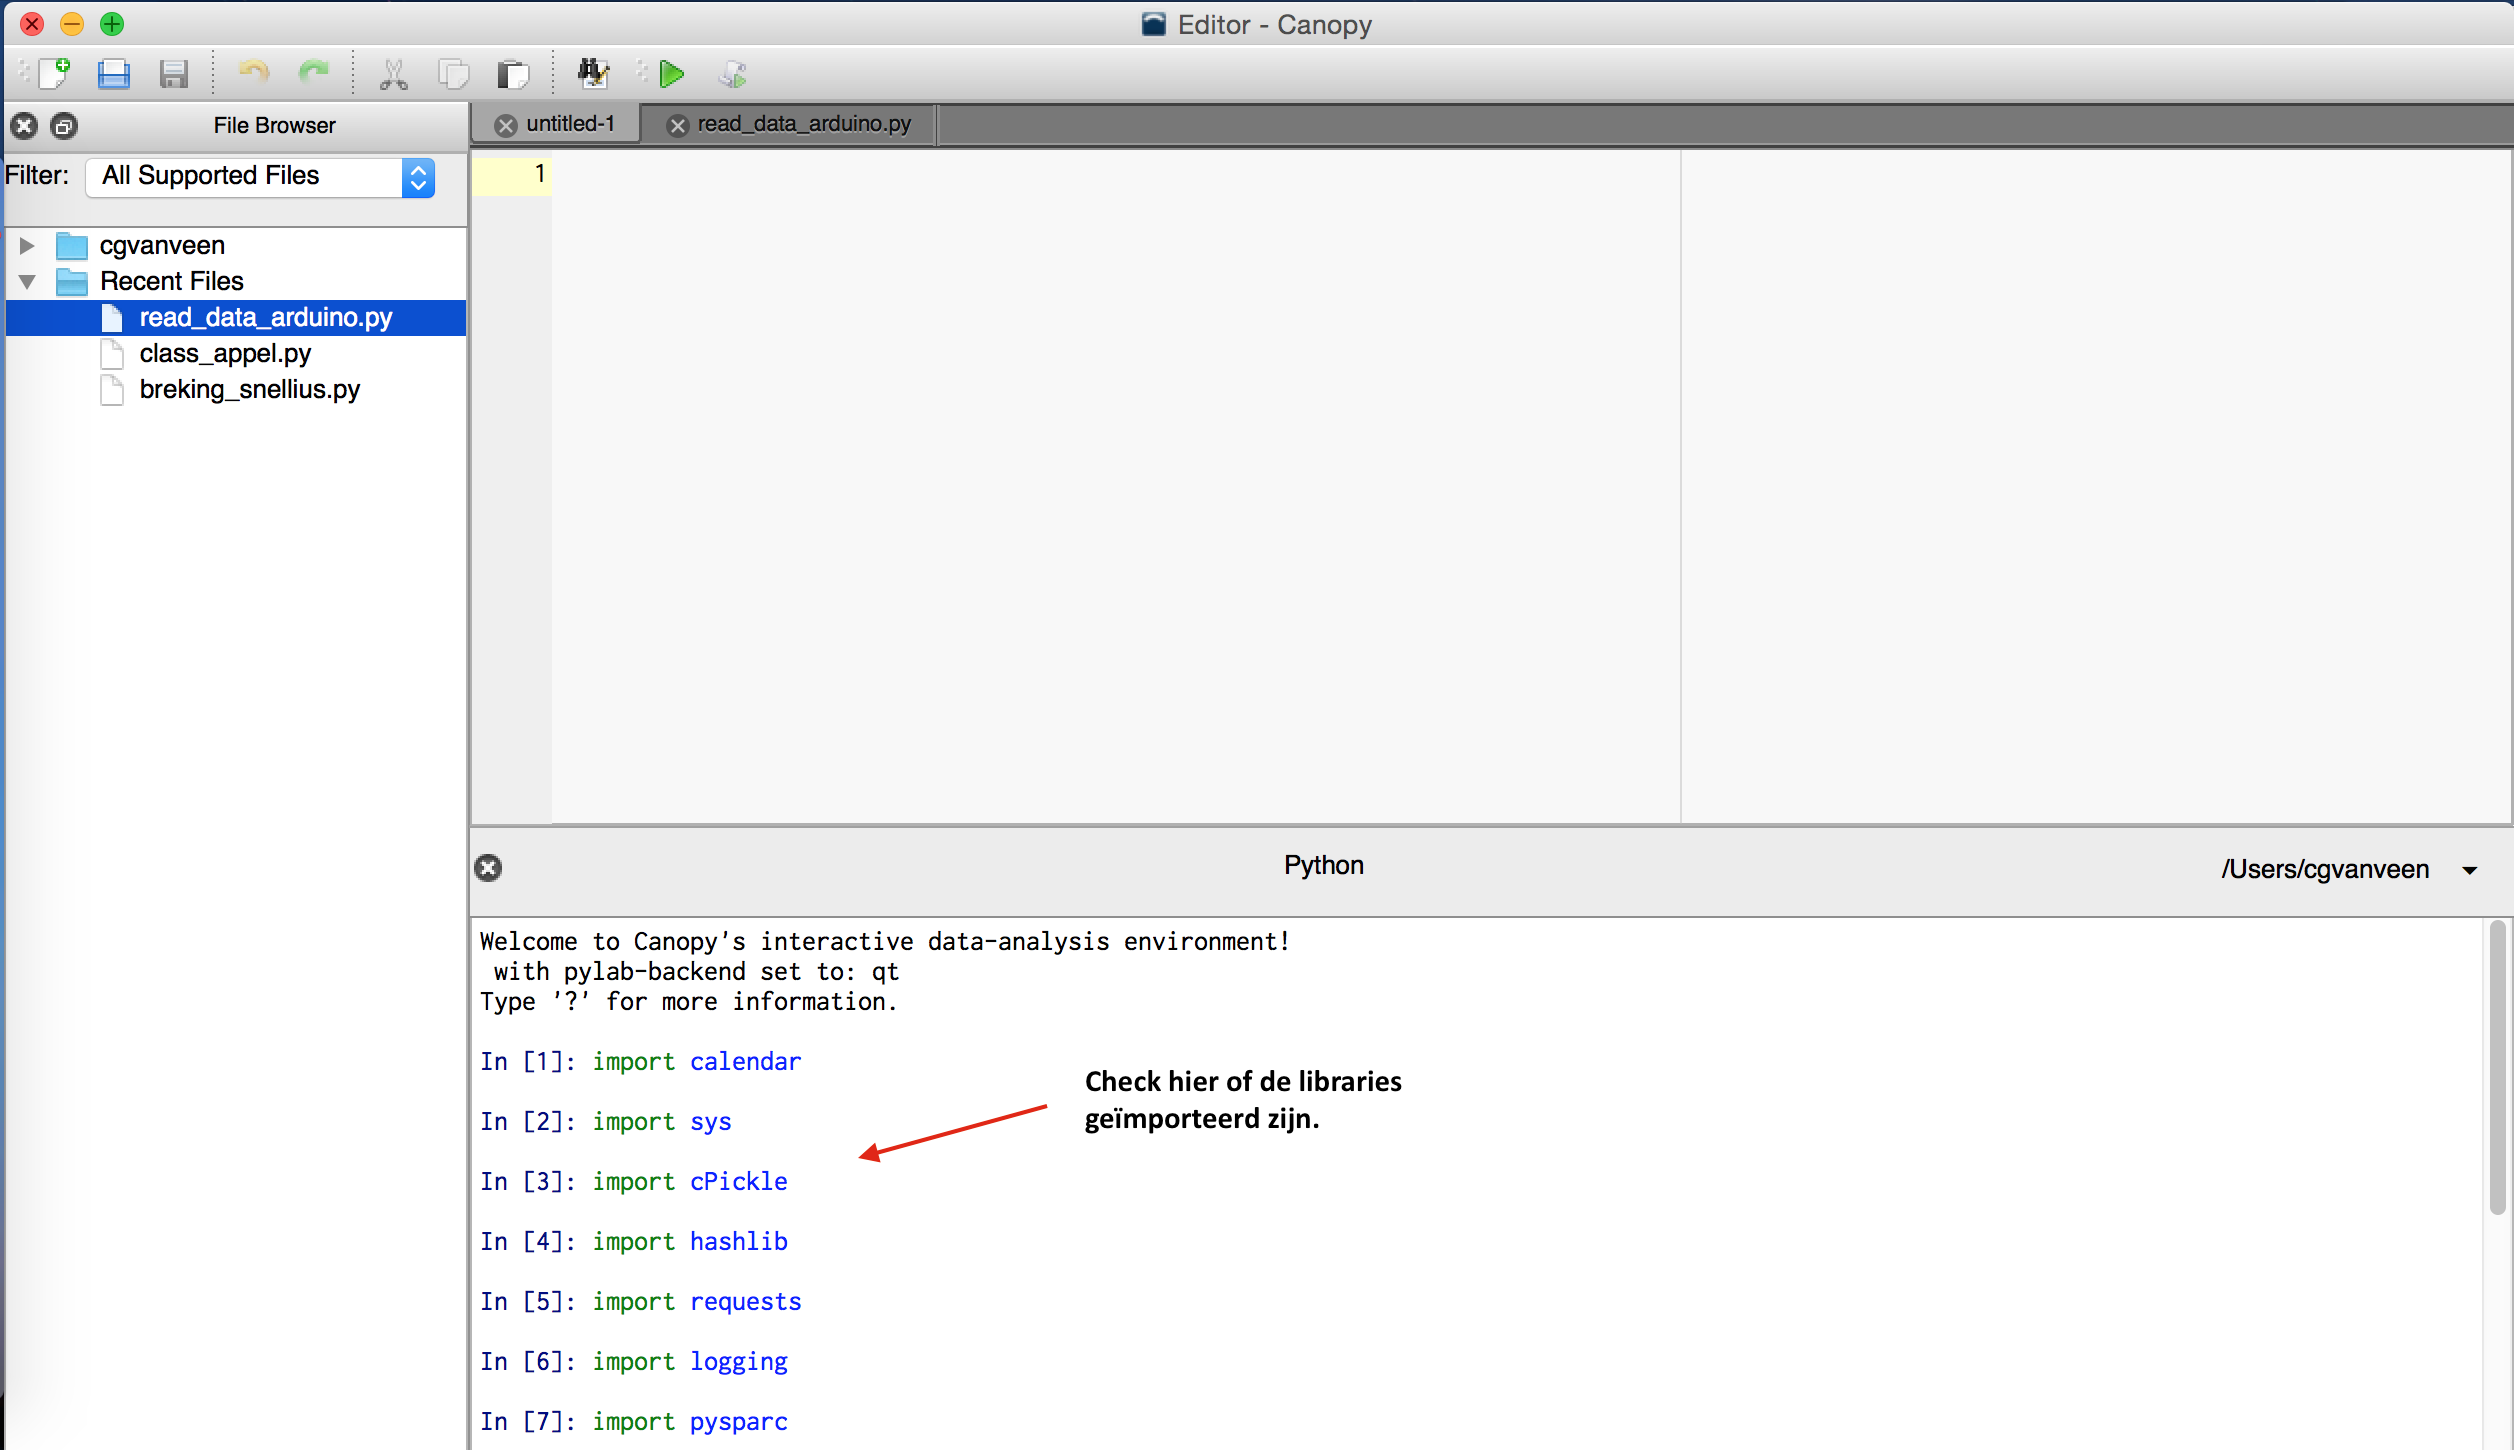
\includegraphics[width=0.80 \textwidth]{Canopy}
    \caption{Venster van Canopy. Anaconda werkt op eenzelfde manier. Hier kun je
    in het interactieve venster invoeren `import ...' en dan enter. Als de library
    niet is gevonden, geeft het programma een foutmelding.}
    \label{fig:canopy1}
\end{figure}

Om te checken of libraries geïmporteerd zijn kun je in Anaconda in het
interactieve venster invoeren: \emph{import ......}. Zie
\figref{fig:canopy1} waarbij hetzelfde is gedaan met Canopy.

Als je geen foutmelding hebt dan is de library geïnstalleerd.
In code 4 kun je zien welke libraries allemaal toegevoegd moeten zijn.

\begin{minted}{python}
# Code 4
import serial
import datetime
import time
import logging
import calendar

import numpy

from pysparc import storage
\end{minted}

Waarschijnlijk moet `pysparc' nog geïnstalleerd worden. Open de terminal van
Anaconda. Wat we gaan doen is een link naar de pysparc module van \hisparc
maken en deze gelijk installeren. type:
\begin{verbatim}
pip install https://github.com/HiSPARC/pysparc/archive/primary.zip
\end{verbatim}

Nu kun je \verb|import pysparc| gebruiken, Zie \figref{fig:canopy1}.


\subsection{Storage backup}

Als de internet verbinding wegvalt dan willen we niet dat de data verloren gaat.
We gebruiken daarom module \emph{pysparc}. Deze gebruikt een database (Redis) om data
op te slaan, totdat er weer een internetverbinding tot stand komt.

- Voor \textbf{windows} ga je naar:
\begin{verbatim}
https://github.com/rgl/redis/downloads
\end{verbatim}

Download de versie van Redis, die je nodig hebt.
Installeer Redis op je computer. Start nu de `command prompt' als administrator.
Run het volgende commando:

\begin{verbatim}
net start redis
\end{verbatim}

Elke keer dat je de (Windows-)computer opnieuw opstart, moet wel Redis opnieuw
opgestart worden.

- Voor de \textbf{Mac}:
Als je `Homebrew' geïnstalleerd hebt dan kun je eenvoudig het volgende
in een terminal intypen: (`Homebrew' is eenvoudig te vinden met Google
en dan te installeren op de Mac.

\begin{verbatim}
brew install redis
\end{verbatim}

Heb je geen Homebrew. Open dan een terminal en type de volgende commando's in.

\begin{enumerate}
    \item curl -O http://download.redis.io/redis-stable.tar.gz
    \item tar -xvzf redis-stable.tar.gz
    \item rm redis-stable.tar.gz
    \item cd redis-stable
    \item make
    \item sudo make install
    \item redis-server
\end{enumerate}

De Redis server is nu geïnstalleerd en gestart.


\subsection{Meten met het weerstation en data opsturen}

Zorg dat je in Arduino het weerprogramma upload naar de Arduino
(bijvoorbeeld met een USB kabel. Haal bij deze procedure het snoertje bij `Rx' op de
Arduino weg.) Bekijk in de Serial monitor of de de data correct wordt
weergegeven. Sluit nu de UART-APC220 module aan op de Arduino en de PC.

Start Redis.

Open nu het Python programma (te vinden op
\url{https://github.com/HiSPARC/weather-arduino}. \verb|Datafromwirelesstodatabase.py|.
Run het programma.
\emph{!Pas op!} Pas dit Python programma eventueel alleen aan in de `class' die in deze
handleiding benoemd is. Dus alleen in de class `Measurement' kun je sensor waarden
toevoegen.

Om te checken of het allemaal werkt draai je het programma in Anaconda. Vul zelf
je \hisparc station nummer in en het paswoord voor dat station. Het paswoord is te krijgen
bij \hisparc door te mailen naar \verb|hisparc@utah.edu|.

Door het Python script wordt alleen het dauwpunt geprint. Dit om te checken
of er nog steeds gemeten wordt. Als het goed is zou het dauwpunt tussen
een waarde van 0-10 moeten liggen. Dit printen kun je als commentaar uitschakelen.

Sluit het internet even af en kijk of na weer inschakelen van het internet weer
data verzonden wordt. Als dat gebeurt is alles klaar voor gebruik.
Werkt dat niet kijk, dan even of Redis opgestart is en run je het programma
nog eens.
Plaats nu je weerstation op het dak bij het station. Na een dag meten kun je
bij de gegevens van het station ook de `weer-grafiekjes' zien. Bekijk ze op
\url{data.hisparc.nl}.
Je eigen weerdata kun je nu altijd online uitlezen met dataretrieval tool. Zie de handleiding
'data retrieval' op \url{https://docs.hisparc.nl/infopakket//}.

\end{document}
